During the training of the model we randomly sampled rotational and translational degrees of freedom of a decoy structure. Ideally, we 
want the score assigned by the model to a decoy to be invariant under these transformations. However Fig \ref{Fig:ScoreDistribution} 
shows that the distribution
of scores under rotations and translations follows the gaussian distribution. The Fig. \ref{Fig:DecoysScoreDistribution} 
shows the distributions of scores for several decoys. We see that the difference between the scores of different decoys is 
bigger than the variance of the score under ratations and translations. However, the overlap between 
the distributions can influence the final results. Therefore, to approximate the average score of a decoy we 
sample the score under random translation and rotation 100 times for each decoy in the test set. The final score is then the average of these 
samples.

\begin{figure}[H]
    \centering
    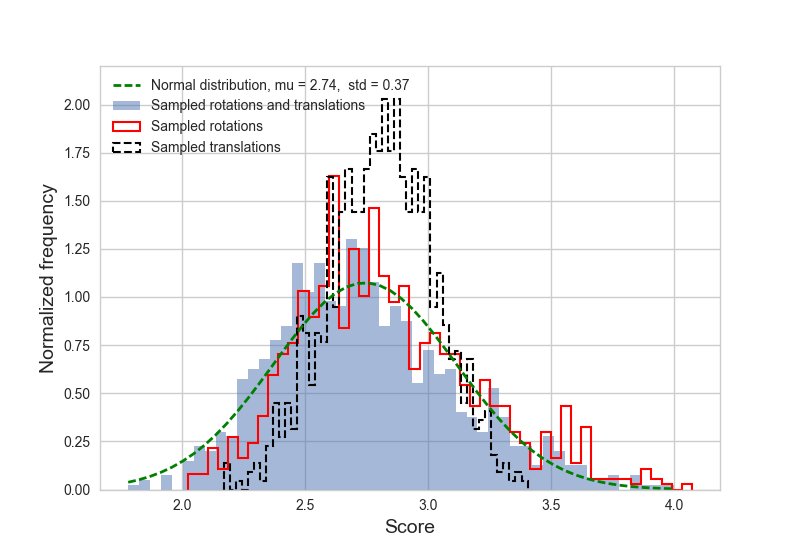
\includegraphics[width=\linewidth]{Fig/sampling_dist.png}
    \caption{The distribution of scores under random translations and rotations of the decoy 
    FALCON\_EnvFold\_TS1 for the target T0832. The distributions 
    os scores under rotations only and translations only are shown with the dashed and solid lines respectively.
    The normal distribution fitted into the sampled scores under both rotations and translations is show with the dashed line.
    \tchanged{ 
    The parameters of the normal distribution are: the average $\mu = 2.74$ and the standard deviation $\sigma = 0.37$.}}
    \label{Fig:ScoreDistribution}
\end{figure}

\begin{figure}[H]
    \centering
    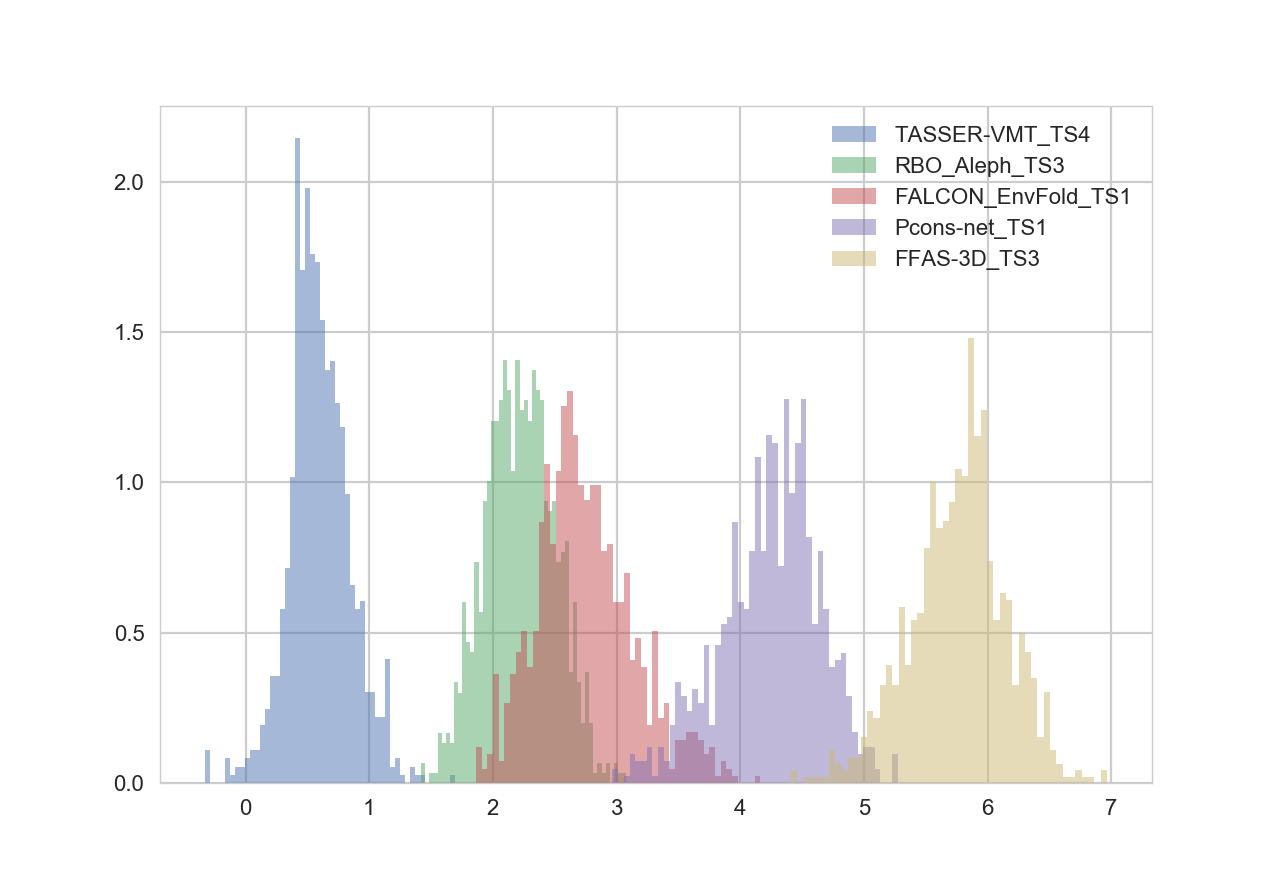
\includegraphics[width=\linewidth]{Fig/decoys_sampling_dist.png}
    \caption{The distribution of scores under random translations and rotations of several decoys for the target T0832. The 
    names arrangement from top to bottom corresponds to the increase of the score.}
    \label{Fig:DecoysScoreDistribution}
\end{figure}
\tchanged{
Table \ref{Tbl:TestResults} shows the comparisson of our model with the state of art methods used for the decoy quality assessement:
ProQ2D,ProQ3D\cite{uziela2017proq3d}, VoroMQA\cite{olechnovivc2017voromqa} and RWPlus\cite{zhang2010novel}.
}
\begin{table}[H]
\begin{center}
\begin{tabular}{ c | c | c | c | c }
    \multicolumn{5}{ c }{Stage 1} \\ \hline

    QA method & Loss & Pearson & Spearmann & Kendall \\
    \hline
    ProQ3D   &0.048 &0.747 &0.658 &0.516 \\
    ProQ2D   &0.068 &0.722 &0.589 &0.456 \\
    \textbf{3DCNN}   &0.071 &0.528 &0.414 &0.318 \\    
    VoroMQA &0.095 &0.621 &0.504 &0.382 \\
    RWplus  &0.128 &0.500 &0.387 &0.291 \\ \hline
    
    \multicolumn{5}{ c }{Stage 2} \\ \hline
    \textbf{3DCNN}   &0.067 &0.420 &0.405 &0.285 \\
    VoroMQA &0.069 &0.444 &0.437 &0.313 \\ 
    ProQ3D   &0.070 &0.450 &0.429 &0.304 \\
    ProQ2D   &0.077 &0.435 &0.418 &0.296 \\
    RWplus  &0.095 &0.202 &0.246 &0.175 \\ \hline

\end{tabular}
    
    \caption {Results of our method(3DCNN) and the other state-of-art quality assessment programs on the CASP11 dataset Stage 1 and 2.
            Table shows the absolute average values of correlation coefficients. The averaging was performed for each target in the 
            dataset. Afterwards all the values were averaged over all the targets.}
    \label{Tbl:TestResults}
\end{center}
\end{table}

Figure \ref{Fig:LossVsECOD} shows the performance of the algorithms depending on the presense in the training set of the structures in the same ECOD 
class. The degree to which the algorithm performs better on the structures closely related to the training ones can indicate 
the proportion of memorization of an algorithm. We see, that our algorithm has the same performance gains for the proteins 
similar to ones in the test set as the VoroMQA and ProQ2D. The algorithm that stands out in this metric is the RWPlus, which 
seems to be indifferent to the homology. However, its performance is also lower than that of the other contenders.

\begin{figure}[H]
    \centering
    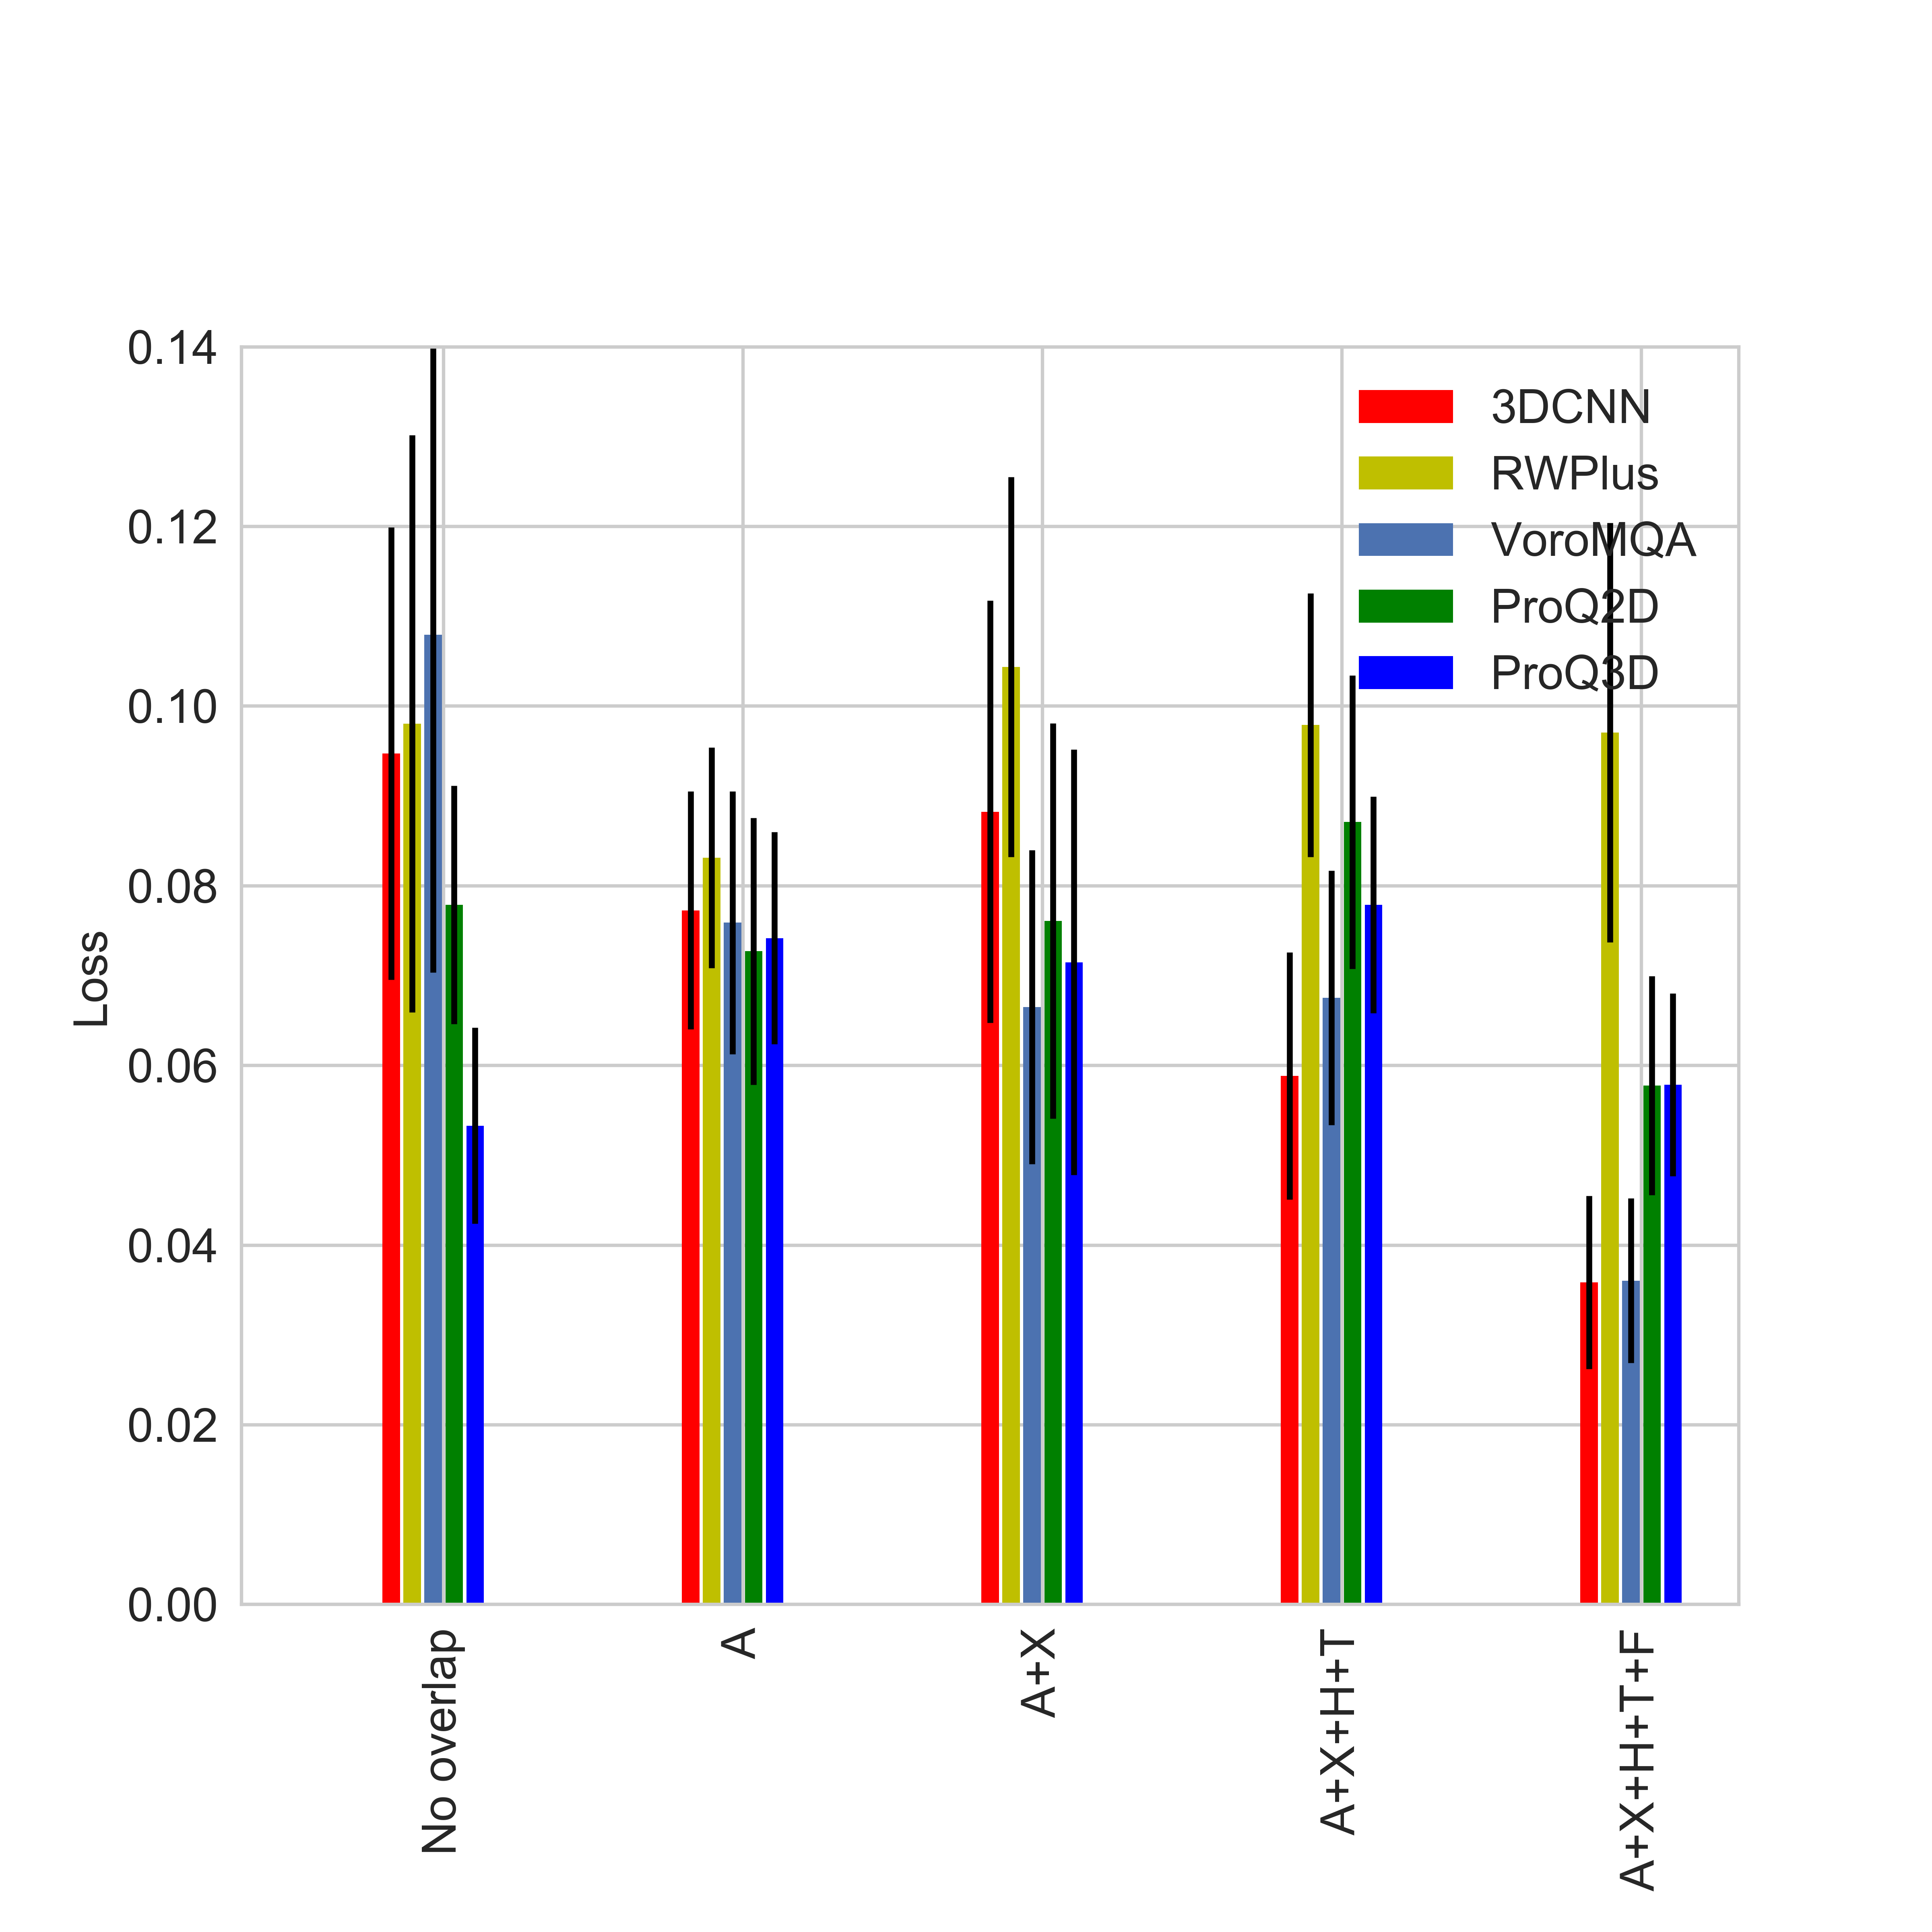
\includegraphics[width=\linewidth]{Fig/LossVsECOD.png}
    \caption{Loss of different QA-algorithms on the subsets of the CASP11 test set Stage2. The subsets are chosen according to the presense in the
    training set of the structures classified into the same ECOD categories.}
    \label{Fig:LossVsECOD}
\end{figure}
